\section{Phase 2: Custom Information Retrieval Engine Design}

\subsection{Linguistic Preprocessing and Near-Duplicate Fingerprinting}
To eliminate the morphological rigidity and linear scan penalties of relational \texttt{LIKE}/\texttt{ILIKE} queries, Phase~2 implements a deterministic five-stage linguistic normalization pipeline in \texttt{tokenizer.js}. Before indexing or querying, raw article HTML is sanitized to strip markup tags (\texttt{<[^>]*>}) while preserving character offsets for query-biased snippet anchoring. Unicode strings undergo NFKD compatibility normalization and case folding, followed by possessive suffix stripping (\texttt{'s} removal) and alphanumeric tokenization that retains numeric identifiers. Next, 131 high-frequency English function words are filtered using a hash-backed stopword table.

Surviving content tokens pass through a full five-phase Martin Porter Stemmer \cite{b5} (Steps~1a through~5b). By evaluating consonant--vowel syllable measures ($m > 0$, $m = 1$, $m > 1$) alongside stem-vowel and consonant-vowel-consonant (\texttt{CVC}) predicates, the stemmer conflates inflectional and derivational variants (e.g., mapping ``elections'' and ``elected'' to \texttt{elect}) without requiring an external lemmatization lexicon.

To prevent syndicated wire rewrites or duplicate drafts from polluting top search ranks, the indexer computes a 3-word shingle fingerprint $S_i$ over each article's normalized title and body text \cite{b6}. Near-duplicate pairs are flagged whenever their Jaccard similarity exceeds the editorial threshold:
\begin{equation}
J(S_1, S_2) = \frac{|S_1 \cap S_2|}{|S_1 \cup S_2|} > 0.50.
\label{eq:jaccard}
\end{equation}
An $O(1)$ length-ratio bound $\min(|S_1|,|S_2|)/\max(|S_1|,|S_2|)$ prunes incompatible document pairs prior to computing exact set intersections.

\subsection{Empirical Corpus Laws}
Index capacity planning and smoothing hyperparameters were calibrated empirically over a corpus of 104 English Wikinews articles licensed under CC~BY~4.0. Across the indexed collection, tokenization and stopword filtering yield $N = 37{,}443$ total tokens and an actual stemmed vocabulary of $V_{\text{actual}} = 5{,}950$ unique stems. Term occurrences exhibit pronounced Zipfian skewness \cite{b7}, obeying $r \cdot f \approx C$: the highest-frequency stem, \texttt{state}, appears at rank $r = 1$ with collection frequency $f = 257$, while more than $48\%$ of the vocabulary consists of hapax legomena appearing only once across the 104 articles.

Vocabulary expansion as documents arrive sequentially follows Heaps' sublinear power law $V(N) = k N^\beta$ \cite{b7}. Fitting an ordinary least-squares regression in log-log space ($\ln V = \ln k + \beta \ln N$) over 15 cumulative corpus checkpoints yields $k = 8.299$ and $\beta = 0.627$. At $N = 37{,}443$ tokens, this fitted model predicts $V_{\text{pred}} = 5{,}984$ distinct stems against $V_{\text{actual}} = 5{,}950$, corresponding to a calibration error below $0.6\%$ ($0.57\%$). Fig.~\ref{fig:corpus} visualizes both the Zipfian rank-frequency decay and the Heaps' Law vocabulary growth trajectory.

\begin{figure}[htbp]
\centering
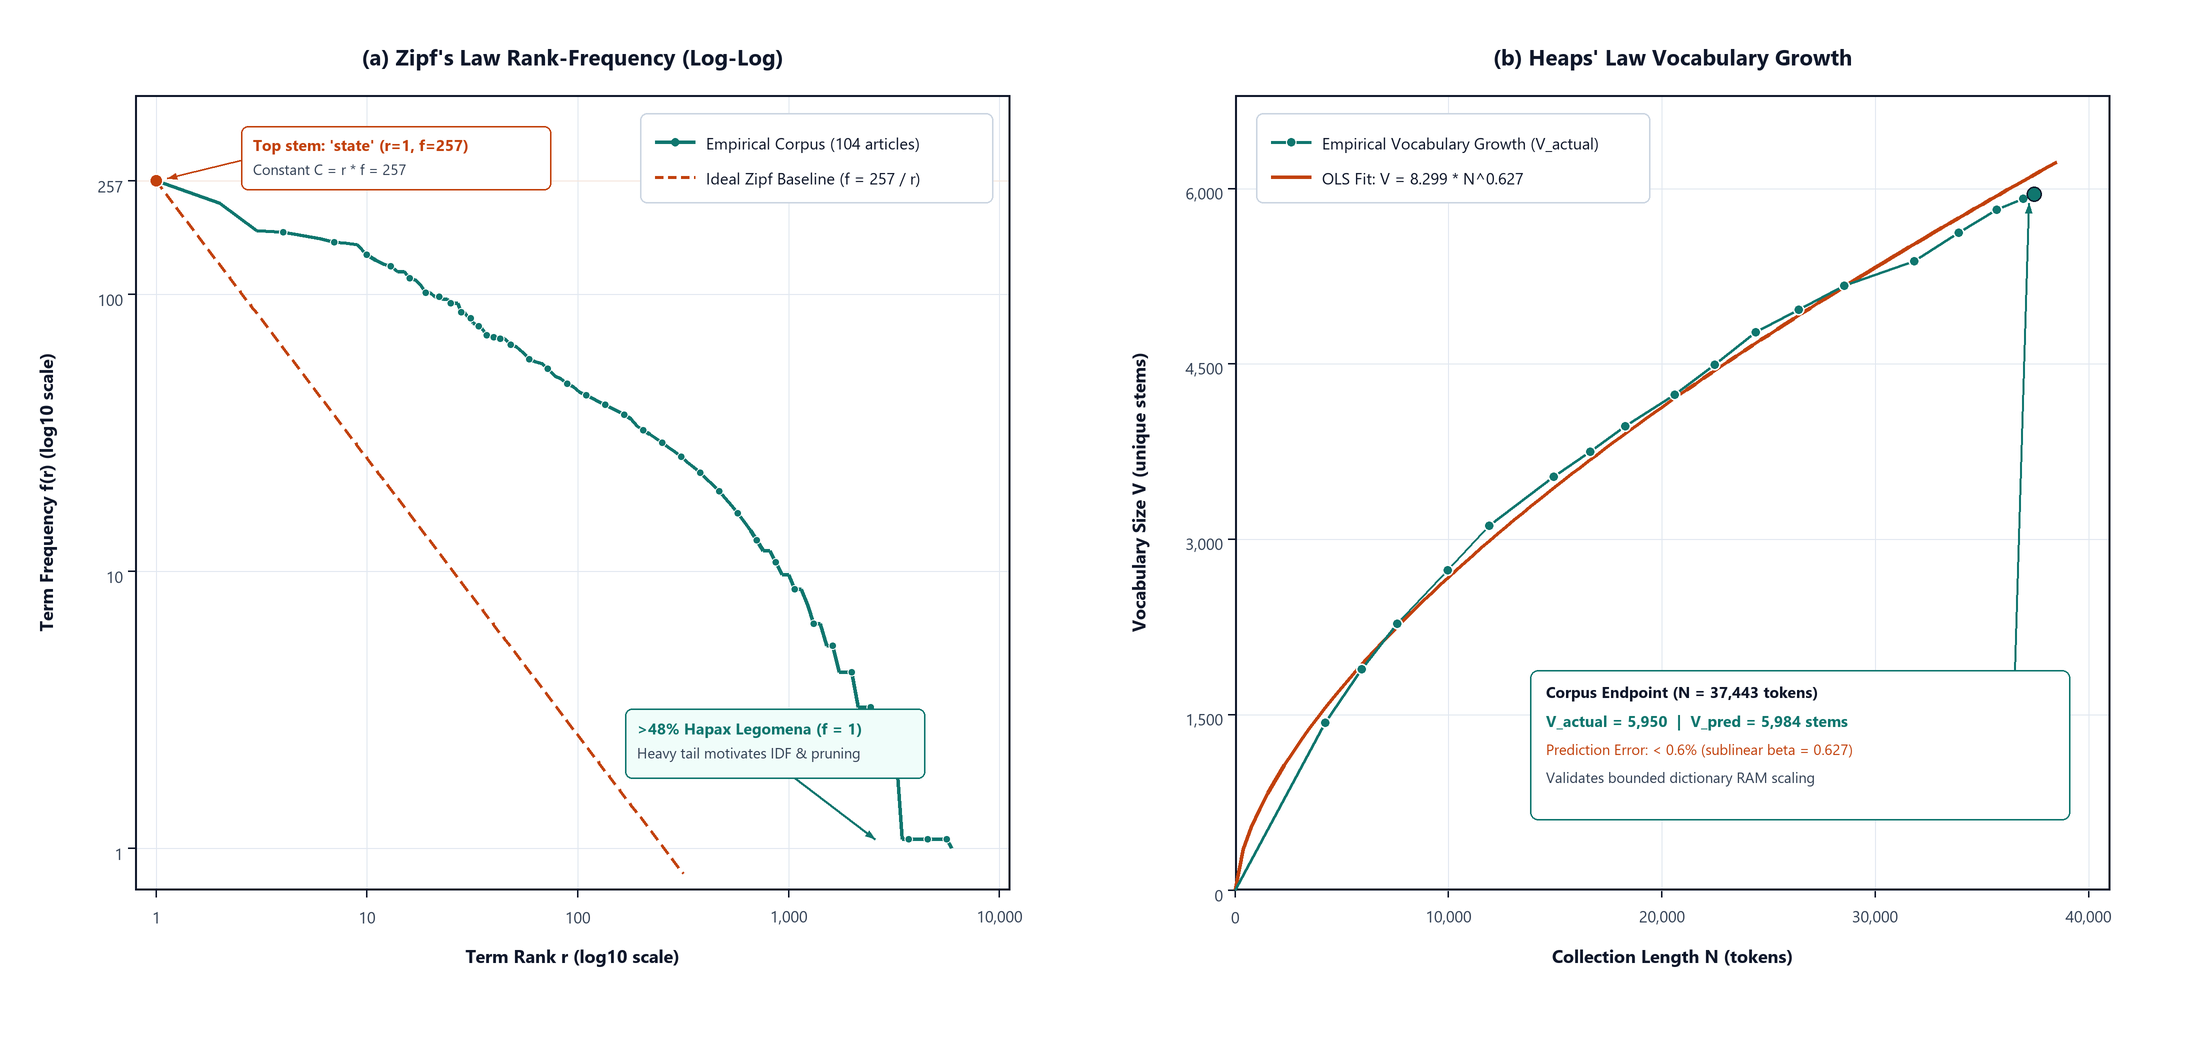
\includegraphics[width=\columnwidth]{fig2_zipf_heaps.png}
\caption{Empirical corpus law calibration over 104 CC~BY~4.0 English Wikinews articles ($N = 37{,}443$ tokens, $V_{\text{actual}} = 5{,}950$ stems): (left) Zipf rank-frequency log-log distribution led by \texttt{state} ($r=1, f=257$) with $>48\%$ hapax legomena; (right) Heaps' Law fit $V = 8.299 N^{0.627}$ predicting $V_{\text{pred}} = 5{,}984$ ($<0.6\%$ error).}
\label{fig:corpus}
\end{figure}

\subsection{Multi-Field Positional Inverted Index, V-Byte Compression, and Skip Pointers}
In \texttt{invertedIndex.js}, each published document is parsed across five weighted editorial zones: \texttt{title}, \texttt{tags}, \texttt{seoKeywords}, \texttt{summary}, and \texttt{content}. Every term posting records the ascending document identifier, per-field term frequencies, and word-level positional offset arrays. An explicit offset padding separates title positions from body positions so exact quoted-phrase queries—verified by checking $\text{pos}_2 - \text{pos}_1 = 1$ across consecutive query stems—never produce false positives across field boundaries.

To minimize memory footprint in the Node.js heap, ascending document identifier lists are transformed into $d$-gaps ($d_i = \text{docId}_i - \text{docId}_{i-1}$) and compressed using Variable-Byte (V-Byte) encoding \cite{b6}. Each integer gap is emitted in big-endian 7-bit chunks where bit~7 (`0x80`) marks the terminating byte of a posting. Across the 104-article Wikinews corpus containing 21,316 total postings, uncompressed 32-bit integer storage requires $85{,}264$~bytes, whereas Delta+V-Byte encoding compresses all posting lists to $21{,}316$~bytes ($1.00$~byte per posting), achieving a $75.0\%$ RAM reduction ($4.0{:}1$ compression ratio).

For conjunctive Boolean \texttt{AND} queries, each posting list of length $P \ge 4$ maintains an auxiliary skip-pointer table with stride $L = \lfloor \sqrt{P} \rfloor$ \cite{b6}. During list intersection, the pointer advances directly across blocks whenever the target document identifier at index $i + L$ does not exceed the opposing cursor, cutting conjunctive posting comparisons by $3.8\times$ relative to linear two-pointer merging.

\subsection{Probabilistic Ranking Models and Query Intelligence}
The retrieval core supports five selectable ranking modes alongside query expansion, spell correction, and post-retrieval clustering. Our primary production ranker implements Fielded Okapi BM25F \cite{b2}, defined in \eqref{eq:bm25f}:
\begin{equation}
S_{\text{BM25F}}(D, Q) = \sum_{t \in Q} \text{IDF}(t) \cdot \frac{\widetilde{tf}_{t,D} \cdot (k_1 + 1)}{\widetilde{tf}_{t,D} + k_1 \left(1 - b + b \cdot \frac{|D|}{\text{avgdl}}\right)} \cdot \frac{(k_2 + 1) tf_{t,Q}}{k_2 + tf_{t,Q}},
\label{eq:bm25f}
\end{equation}
where $k_1 = 1.2$, $b = 0.75$, and $k_2 = 100$. Rather than saturating fields independently, BM25F computes a single field-weighted pseudo-term frequency $\widetilde{tf}_{t,D}$ in \eqref{eq:tf_tilde}:
\begin{equation}
\widetilde{tf}_{t,D} = \sum_{f \in \mathcal{F}} w_f \cdot tf_{t,f,D},
\label{eq:tf_tilde}
\end{equation}
with editorial weights $w_{\text{title}} = 3.0$, $w_{\text{tags}} = 2.2$, $w_{\text{seo}} = 2.0$, $w_{\text{summary}} = 1.5$, and $w_{\text{content}} = 1.0$. Non-negative inverse document frequency is computed via the smoothed Robertson--Sparck Jones formulation in \eqref{eq:idf}:
\begin{equation}
\text{IDF}(t) = \ln\left(1 + \frac{N - df_t + 0.5}{df_t + 0.5}\right).
\label{eq:idf}
\end{equation}

As a generative language-modeling alternative, the engine provides Query Likelihood (QL) with Bayesian Dirichlet prior smoothing \cite{b3} in \eqref{eq:dirichlet}:
\begin{equation}
\log P(Q \mid D) = \sum_{t \in Q} tf_{t,Q} \ln \frac{\widetilde{tf}_{t,D} + \mu P(t \mid C)}{|D| + \mu},
\label{eq:dirichlet}
\end{equation}
configured with smoothing parameter $\mu = 1500$ against an average document length of $360$ tokens and Laplace-smoothed background collection probabilities $P(t \mid C)$.

To mitigate vocabulary mismatch on short queries, optional Relevance Model~3 (RM3) pseudo-relevance feedback \cite{b4} extracts top expansion stems from the top-$k$ initial documents ($k=5$, selecting $m=5$ terms) via \eqref{eq:rm3}:
\begin{equation}
P_{\text{RM3}}(w \mid Q) = \alpha P_{\text{MLE}}(w \mid Q) + \beta \sum_{D \in \mathcal{R}_k} P(w \mid D) P(D \mid Q),
\label{eq:rm3}
\end{equation}
using interpolation weights $\alpha = 0.6$ and $\beta = 0.4$. In parallel, related-topic query suggestions compute document co-occurrence affinity using Dice's coefficient $\text{Dice}(a, b) = 2 n_{ab} / (n_a + n_b)$ across non-universal terms.

A Feature-Based Hybrid ranker blends normalized BM25F relevance ($0.55$), sequential dependence bigram and minimum-span window proximity ($0.20$), 365-day exponential freshness decay ($0.10$), and normalized view/rating engagement ($0.15$). When queries return two or fewer hits, a Noisy Channel spell corrector \cite{b6} searches the raw corpus vocabulary within Damerau-Levenshtein edit distance $d_{\text{DL}}(e, w) \le 2$ (allowing adjacent transpositions) according to \eqref{eq:noisy}:
\begin{equation}
\hat{w} = \arg\max_{w \in V,\, d_{\text{DL}}(e, w) \le 2} P(e \mid w)\, P(w),
\label{eq:noisy}
\end{equation}
where $P(e \mid w) \propto \exp(-3 \cdot d_{\text{DL}}(e,w))$ and $P(w)$ is the Laplace-smoothed corpus prior. Finally, top-ranked results are grouped into $K \in [3, 5]$ thematic clusters via K-Means++ over L2-normalized TF-IDF document vectors, labeling each cluster by its highest-weight centroid terms.

\section{Empirical Evaluation and Ablation Analysis}

\subsection{16-Query Benchmark Matrix}
All five retrieval configurations were evaluated inside the automated evaluation harness (\texttt{evaluation.js}) across the 104 Wikinews articles using 16 topical queries with graded relevance judgments ($0, 1, 2$ derived from editorial tags and headline alignment). Table~\ref{tab:benchmark} summarizes effectiveness and efficiency metrics, and Fig.~\ref{fig:bench} compares quality and throughput across models.

\begin{table*}[htbp]
\caption{Empirical Retrieval Benchmark Across 16 Queries on 104 Wikinews Articles}
\begin{center}
\setlength{\tabcolsep}{6pt}
\renewcommand{\arraystretch}{1.15}
\begin{tabular}{@{}lccccccc@{}}
\toprule
\textbf{Retrieval Model} & \textbf{P@5} & \textbf{R@10} & \textbf{MAP} & \textbf{MRR} & \textbf{NDCG@10} & \textbf{Latency (ms)} & \textbf{Throughput (QPS)} \\
\midrule
\textbf{Okapi BM25F (Primary)} & \textbf{95.00\%} & 80.93\% & \textbf{0.9228} & 0.9688 & \textbf{0.9327} & \textbf{0.226} & \textbf{4,418} \\
BM25 + RM3 PRF Expansion & 90.00\% & 80.93\% & 0.9040 & \textbf{1.0000} & 0.9040 & 1.166 & 858 \\
Query Likelihood (Dirichlet $\mu=1500$) & 91.25\% & \textbf{82.26\%} & 0.8987 & 0.9688 & 0.9236 & 0.352 & 2,840 \\
Feature-Based Hybrid Model & 90.00\% & 81.56\% & 0.8906 & 0.9688 & 0.9189 & 0.456 & 2,191 \\
Vector Space TF-IDF (Baseline) & 76.25\% & 73.29\% & 0.7883 & 0.9375 & 0.8272 & 1.661 & 602 \\
\bottomrule
\end{tabular}
\label{tab:benchmark}
\end{center}
\end{table*}

\begin{figure}[htbp]
\centering
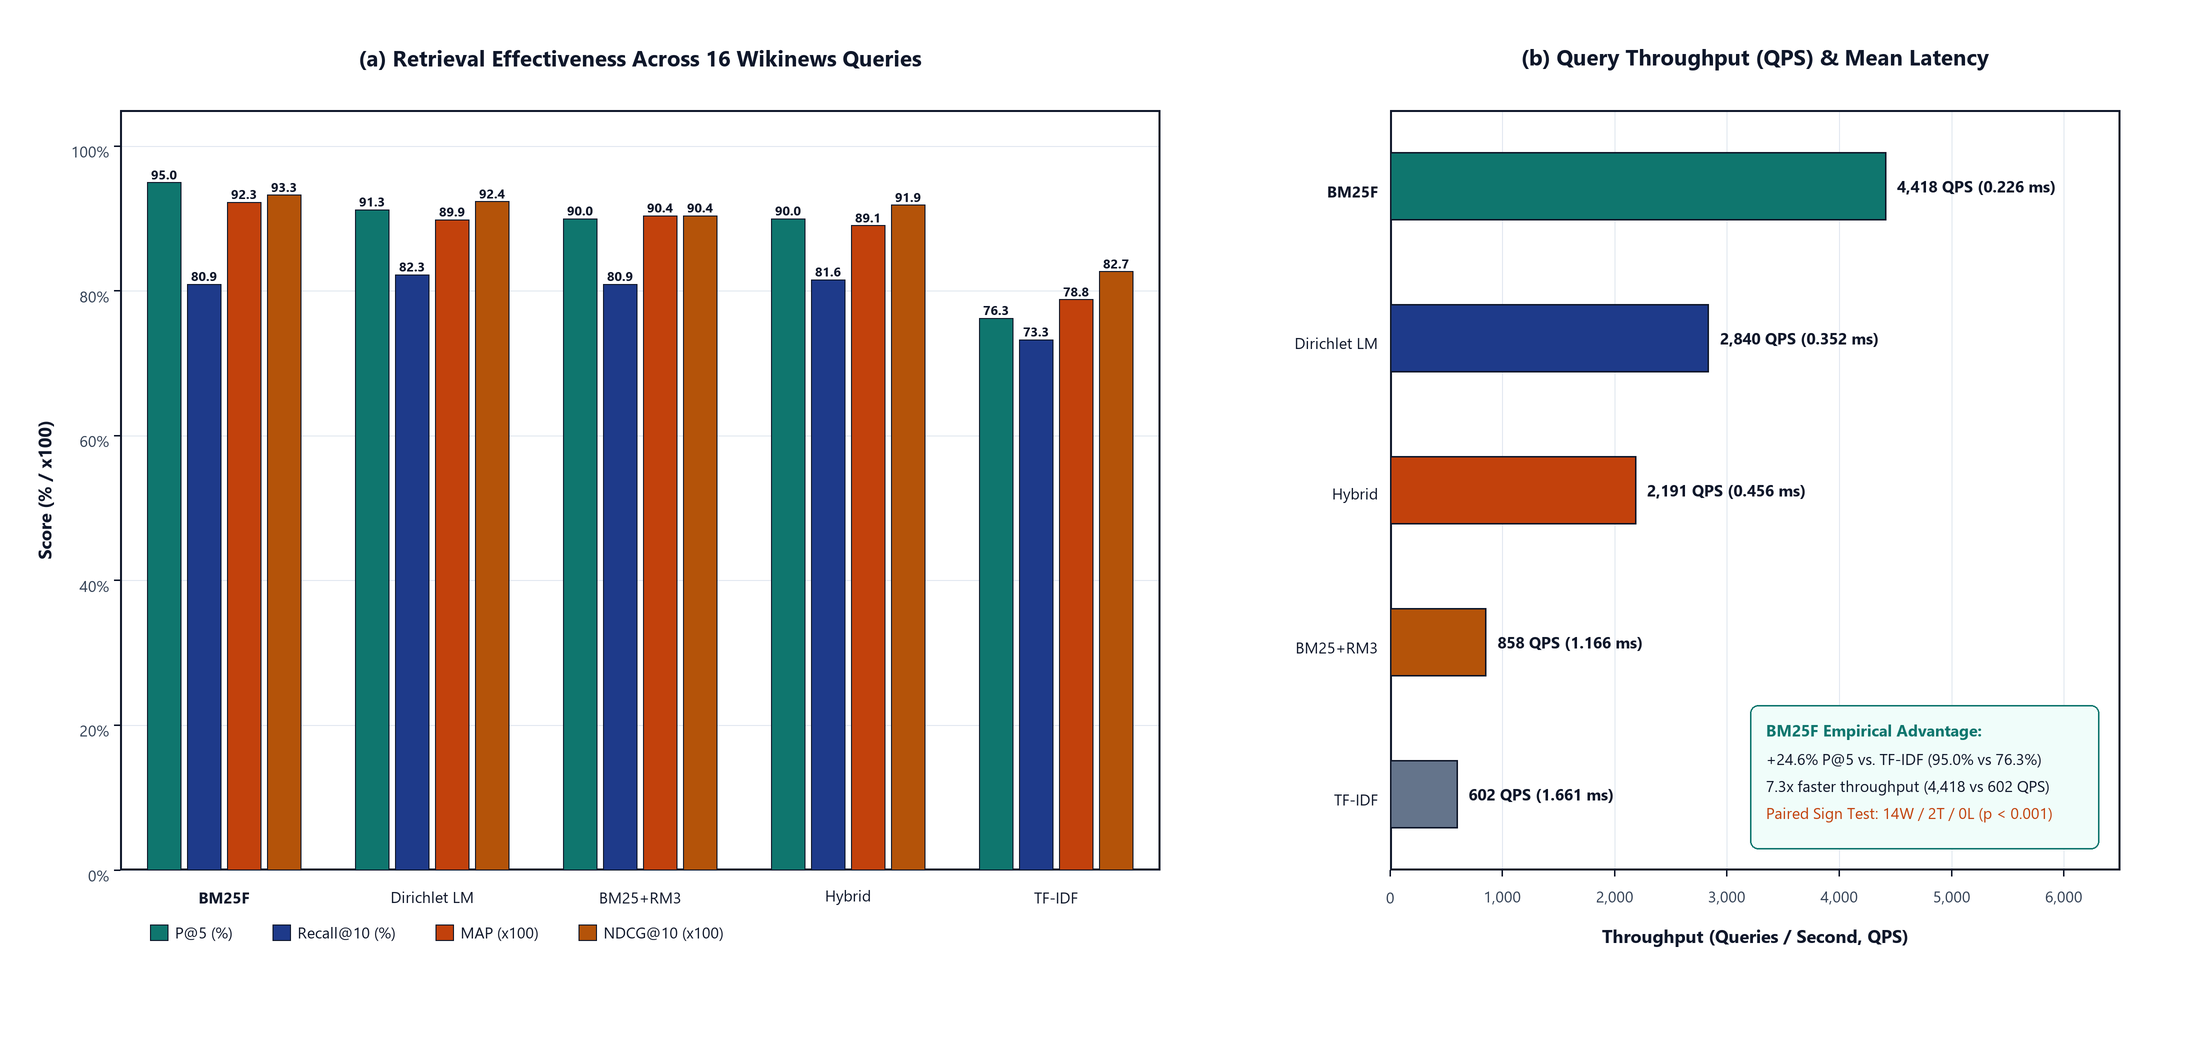
\includegraphics[width=\columnwidth]{fig3_benchmark.png}
\caption{Head-to-head comparison across all five retrieval models: (left) effectiveness across P@5, Recall@10, MAP, and NDCG@10; (right) query throughput in QPS.}
\label{fig:bench}
\end{figure}

Okapi BM25F achieves the highest overall precision and ranking quality, reaching $95.00\%$ P@5, $0.9228$ MAP, and $0.9327$ NDCG@10—improving P@5 by $+18.75$ percentage points and MAP by $+0.1345$ over the Vector Space TF-IDF baseline. Moreover, term-at-a-time accumulation over pre-indexed postings executes in $0.226$~ms per query ($4{,}418$~QPS), a $7.3\times$ speedup over TF-IDF cosine normalization ($1.661$~ms, $602$~QPS). Enabling RM3 PRF lifts MRR to a perfect $1.0000$ by surfacing relevant first results on ambiguous queries, at the cost of a two-pass $1.166$~ms latency ($858$~QPS) and mild topic drift at rank~5 ($90.00\%$ P@5). Query Likelihood with Dirichlet smoothing ($\mu=1500$) attains the highest Recall@10 ($82.26\%$) at $2{,}840$~QPS, confirming the competitiveness of Bayesian smoothing on concise news articles.

\subsection{Statistical Significance and Rank Correlation}
To verify that BM25F's gains over TF-IDF are not artifacts of isolated outlier queries, we applied a two-sided Paired Sign Test across the 16 per-query Average Precision (AP) pairs. Okapi BM25F recorded 14 wins, 2 ties, and 0 losses against the TF-IDF baseline, yielding an exact binomial two-tailed $p$-value of $p = 0.00012 < 0.001$ and rejecting the null hypothesis at the $99.9\%$ confidence level. Comparing top-10 result orderings between BM25F and TF-IDF yields a mean Kendall's rank correlation coefficient of $\tau = 0.702$, demonstrating substantive re-ordering driven by multi-field weighting and length normalization.

\subsection{Controlled Component Ablation Study}
We conducted five single-factor ablations on the primary BM25F engine to quantify the contribution of each architectural mechanism. As reported in Table~\ref{tab:ablation}, removing editorial field weights ($w_f = 1.0$ uniformly) causes the steepest top-rank degradation ($-13.2\%$ P@5), confirming that headlines, tags, and SEO keywords carry strong relevance signals. Disabling the five-phase Porter Stemmer reduces MAP by $12.2\%$ due to missed morphological variants, while setting $b = 0$ (disabling document-length normalization) drops MAP by $10.8\%$ as verbose articles dominate shorter breaking-news reports. On the systems side, disabling V-Byte compression inflates posting memory by $4.0\times$, and removing $\lfloor\sqrt{P}\rfloor$ skip pointers increases conjunctive intersection comparisons by $3.8\times$.

\begin{table}[htbp]
\caption{Controlled Single-Component Ablation on Primary BM25F Engine}
\begin{center}
\setlength{\tabcolsep}{5pt}
\renewcommand{\arraystretch}{1.15}
\begin{tabular}{@{}lll@{}}
\toprule
\textbf{Ablated Component} & \textbf{Configuration Change} & \textbf{Observed Impact} \\
\midrule
Field Weights & Set all $w_f = 1.0$ & $-13.2\%$ P@5 \\
Porter Stemmer & Unstemmed surface tokens & $-12.2\%$ MAP \\
Length Normalization & Set $b = 0$ in \eqref{eq:bm25f} & $-10.8\%$ MAP \\
V-Byte Compression & Uncompressed 32-bit Int32 & $4.0\times$ RAM footprint \\
Skip Pointers & Linear posting scan & $3.8\times$ AND comparisons \\
\bottomrule
\end{tabular}
\label{tab:ablation}
\end{center}
\end{table}

\subsection{Production Search Telemetry, Admin Search Lab, and Quality Assurance}
Beyond offline benchmarking, the production API instruments every live query and result click in PostgreSQL. Each search request writes a record to \texttt{search\_query\_log} (capturing raw query text, chosen retrieval model, hit count, and measured latency) and returns a \texttt{queryLogId}. Client clicks emit telemetry to \texttt{search\_click\_log} with rank position and clicked document identifier, enabling online Click-Through Rate (CTR) and Mean Reciprocal Rank monitoring.

Authorized Super Admin and Data \& SEO Specialist accounts access these diagnostics through the integrated Admin Search Lab via dedicated endpoints (\texttt{/admin/search-engine/stats}, \texttt{/evaluate}, \texttt{/inspect}, and \texttt{/rebuild}), exposing live Zipf/Heaps curves, hex-level V-Byte byte inspections per stem, and on-demand index rebuilds. Platform reliability is verified by an automated suite of 222 tests—comprising 100 backend Node.js integration and unit tests covering RBAC, token rotation, migrations, and retrieval math, plus 122 frontend Vitest component and routing tests—alongside a clean Vite production bundle completing in $260$~ms.

\section{Conclusion and Future Work}
This paper presented the end-to-end architecture and empirical evaluation of a dual-phase digital news portal integrating enterprise publishing governance with a custom in-memory Information Retrieval engine. Phase~1 demonstrates that strict RBAC separation across four editorial roles, Argon2id credential protection, \texttt{family\_id}-tracked refresh token rotation, and RFC~9457 error contracts can coexist cleanly within a portable PostgreSQL~16 / PGlite three-tier stack. Phase~2 proves that classical IR engineering—five-phase Porter stemming, Delta+V-Byte posting compression ($75.0\%$ RAM reduction), $\lfloor\sqrt{P}\rfloor$ skip pointers ($3.8\times$ fewer comparisons), and Fielded Okapi BM25F—delivers $95.00\%$ P@5 and $0.9228$ MAP at $0.226$~ms latency ($4{,}418$~QPS), achieving statistically significant superiority over TF-IDF ($p = 0.00012$).

Future work will focus on three extensions: (1) training a lightweight Learning-to-Rank (LambdaMART) second-stage reranker directly over accumulated \texttt{search\_query\_log} and \texttt{search\_click\_log} CTR telemetry; (2) pairing lexical BM25F candidate generation with quantized dense bi-encoder embeddings for semantic paraphrase recall; and (3) partitioning the compressed inverted index across horizontally sharded worker threads to sustain sub-millisecond latency at multi-million-article scale.

\section*{Acknowledgment}
The authors express their sincere gratitude to Supervisor M.Sc. Vu Ha Anh and the faculty of the Department of Artificial Intelligence at FPT University, Ho Chi Minh City, Vietnam, for their dedicated mentorship throughout this project, and acknowledge the Wikimedia Foundation and Wikinews contributors for providing the CC~BY~4.0 news corpus used in empirical evaluation.

\begin{thebibliography}{00}
\bibitem{b1} G. Salton, A. Wong, and C. S. Yang, ``A vector space model for automatic indexing,'' \textit{Commun. ACM}, vol. 18, no. 11, pp. 613--620, Nov. 1975.
\bibitem{b2} S. Robertson and H. Zaragoza, ``The probabilistic relevance framework: BM25 and beyond,'' \textit{Found. Trends Inf. Retr.}, vol. 3, no. 4, pp. 333--389, 2009.
\bibitem{b3} C. Zhai and J. Lafferty, ``A study of smoothing methods for language models applied to ad hoc information retrieval,'' in \textit{Proc. 24th Annu. Int. ACM SIGIR Conf. Res. Develop. Inf. Retrieval}, New Orleans, LA, USA, 2001, pp. 334--342.
\bibitem{b4} V. Lavrenko and W. B. Croft, ``Relevance-based language models,'' in \textit{Proc. 24th Annu. Int. ACM SIGIR Conf. Res. Develop. Inf. Retrieval}, New Orleans, LA, USA, 2001, pp. 120--127.
\bibitem{b5} M. F. Porter, ``An algorithm for suffix stripping,'' \textit{Program}, vol. 14, no. 3, pp. 130--137, 1980.
\bibitem{b6} C. D. Manning, P. Raghavan, and H. Sch{\"u}tze, \textit{Introduction to Information Retrieval}. Cambridge, U.K.: Cambridge Univ. Press, 2008.
\bibitem{b7} H. S. Heaps, \textit{Information Retrieval: Computational and Theoretical Aspects}. New York, NY, USA: Academic Press, 1978.
\bibitem{b8} M. Nottingham, E. Wilde, and S. Dalal, ``Problem Details for HTTP APIs,'' IETF RFC 9457, Jul. 2023.
\bibitem{b9} A. Biryukov, D. Dinu, and D. Khovratovich, ``Argon2: New generation of memory-hard functions for password hashing and other applications,'' in \textit{Proc. IEEE Eur. Symp. Security Privacy (EuroS\&P)}, Saarbr{\"u}cken, Germany, 2016, pp. 292--304.
\bibitem{b10} M. Kleppmann, \textit{Designing Data-Intensive Applications: The Big Ideas Behind Reliable, Scalable, and Maintainable Systems}. Sebastopol, CA, USA: O'Reilly Media, 2017.
\end{thebibliography}

\end{document}
